\documentclass[a4paper,12pt]{article}
\usepackage{amsmath,amssymb}
\usepackage[russian]{babel}
\usepackage[utf8]{inputenc}
\usepackage[T2A]{fontenc}
\usepackage{geometry}
\usepackage{listings}
\usepackage{xcolor}
\usepackage{float}
\usepackage{graphicx}
\usepackage{booktabs}
\usepackage{amsopn}
\usepackage{array}
\usepackage{longtable}
\geometry{margin=1.5cm}

\definecolor{intj-bg}{HTML}{2B2B2B}
\definecolor{intj-key}{HTML}{CC7832}
\definecolor{intj-str}{HTML}{6A8759}
\definecolor{intj-comm}{HTML}{808080}
\definecolor{intj-id}{HTML}{A9B7C6}

\lstdefinestyle{intellij}{
  language=Python,
  backgroundcolor=\color{intj-bg},
  basicstyle=\ttfamily\footnotesize\color{intj-id},
  keywordstyle=\color{intj-key}\bfseries,
  stringstyle=\color{intj-str},
  commentstyle=\itshape\color{intj-comm},
  numberstyle=\color{intj-comm}\tiny,
  numbers=left,
  stepnumber=1,
  frame=single,
  rulecolor=\color{intj-comm},
  showstringspaces=false,
  breaklines=true,
  tabsize=4
}

\begin{document}

\begin{figure}[h]
    \centering
    \begin{minipage}{0.45\linewidth}
        \centering
        
\includegraphics[width=\linewidth]{slogan_chernyy}
    \end{minipage}
    \hfill
    \begin{minipage}{0.45\linewidth}
        \centering
        
\includegraphics[width=\linewidth]{cs-logo}
    \end{minipage}
\end{figure}

\begin{table}[htbp]
    \centering
    \begin{tabular}{lrlr}
        Группа & \qquad \qquad P3219 & К работе допущен & \qquad\qquad\qquad\qquad\qquad\qquad \\
        \cmidrule{2-2}\cmidrule{4-4}
        Студент & \qquad \qquad Ануфриев А.С. & Работа выполнена & \qquad\qquad\qquad\qquad\qquad\qquad \\
        \cmidrule{2-2}\cmidrule{4-4}
        Преподаватель & \qquad \qquad Зинченко А.А. & Отчет принят & \qquad\qquad\qquad\qquad\qquad\qquad \\
        \cmidrule{2-2}\cmidrule{4-4}
    \end{tabular}
\end{table}

\vspace{1.5cm}
\begin{center}
    \LARGE
    Вычислительная математика \\[8pt]
    Отчёт по лабораторной работе № 4 \\[6pt]
    \textbf{Аппроксимация функции методом наименьших квадратов} \\[6pt]
    Вариант 2
\end{center}

\vspace{8cm}
\begin{center}
    2026 год \\ Санкт-Петербург
\end{center}

\newpage
\tableofcontents

\newpage

% -------------------------------------------------------
\section{Цель работы}
% -------------------------------------------------------

Найти функцию, являющуюся наилучшим приближением заданной табличной функции по методу наименьших квадратов.

\textbf{Вариант 2.} Функция:
\[
    y = \frac{15x}{x^4 + 2}, \qquad x \in [0,\,4], \quad h = 0{,}4.
\]

% -------------------------------------------------------
\section{Рабочие формулы метода}
% -------------------------------------------------------

\subsection{Постановка задачи аппроксимации}

Пусть дана таблица значений $(x_i, y_i)$, $i = 1,\ldots,n$. Требуется найти функцию $\varphi(x)$, которая наилучшим образом приближает исходные данные.

В методе наименьших квадратов (МНК) ищется функция, минимизирующая сумму квадратов отклонений:
\[
    S = \sum_{i=1}^{n} \varepsilon_i^2 = \sum_{i=1}^{n} [\varphi(x_i) - y_i]^2 \;\longrightarrow\; \min.
\]

\subsection{Полиномиальная аппроксимация}

Аппроксимирующая функция — многочлен степени $m$:
\[
    \varphi(x) = a_0 + a_1 x + a_2 x^2 + \cdots + a_m x^m.
\]
Коэффициенты $a_0, \ldots, a_m$ находятся из системы нормальных уравнений:
\[
\begin{pmatrix}
n & \sum x_i & \sum x_i^2 & \cdots & \sum x_i^m \\
\sum x_i & \sum x_i^2 & \sum x_i^3 & \cdots & \sum x_i^{m+1} \\
\vdots & \vdots & \vdots & \ddots & \vdots \\
\sum x_i^m & \sum x_i^{m+1} & \sum x_i^{m+2} & \cdots & \sum x_i^{2m}
\end{pmatrix}
\begin{pmatrix} a_0 \\ a_1 \\ \vdots \\ a_m \end{pmatrix}
=
\begin{pmatrix} \sum y_i \\ \sum x_i y_i \\ \vdots \\ \sum x_i^m y_i \end{pmatrix}.
\]

\subsubsection{Линейная аппроксимация ($m=1$): $\varphi(x) = ax + b$}

Система двух уравнений:
\[
\begin{cases}
a S_{XX} + b S_X = S_{XY}, \\
a S_X + b n = S_Y,
\end{cases}
\]
где $S_X = \sum x_i$, $S_{XX} = \sum x_i^2$, $S_Y = \sum y_i$, $S_{XY} = \sum x_i y_i$.

По правилу Крамера:
\[
    \Delta = S_{XX}\cdot n - S_X^2, \qquad
    a = \frac{S_{XY}\cdot n - S_X\cdot S_Y}{\Delta}, \qquad
    b = \frac{S_{XX}\cdot S_Y - S_X\cdot S_{XY}}{\Delta}.
\]

\subsubsection{Квадратичная аппроксимация ($m=2$): $\varphi(x) = a_0 + a_1 x + a_2 x^2$}

Система трёх уравнений:
\[
\begin{cases}
a_0 n + a_1 \sum x_i + a_2 \sum x_i^2 = \sum y_i, \\
a_0 \sum x_i + a_1 \sum x_i^2 + a_2 \sum x_i^3 = \sum x_i y_i, \\
a_0 \sum x_i^2 + a_1 \sum x_i^3 + a_2 \sum x_i^4 = \sum x_i^2 y_i.
\end{cases}
\]

\subsection{Нелинейные функции (линеаризация)}

\begin{itemize}
    \item \textbf{Экспоненциальная}: $\varphi(x) = a e^{bx}$.
    Линеаризация: $\ln\varphi = \ln a + bx$, далее линейный МНК по $(x, \ln y)$.
    Возврат: $a = e^A$, $b = B$.

    \item \textbf{Степенная}: $\varphi(x) = a x^b$.
    Линеаризация: $\ln\varphi = \ln a + b\ln x$, МНК по $(\ln x, \ln y)$.
    Возврат: $a = e^A$, $b = B$.

    \item \textbf{Логарифмическая}: $\varphi(x) = a\ln x + b$.
    Линеаризация: $X = \ln x$, МНК по $(X, y)$.
\end{itemize}

\subsection{Метрики качества}

\textbf{Среднеквадратическое отклонение:}
\[
    \delta = \sqrt{\frac{\sum_{i=1}^{n}(\varphi(x_i) - y_i)^2}{n}}.
\]
Наилучшая аппроксимирующая функция — та, для которой $\delta$ минимально.

\textbf{Коэффициент детерминации:}
\[
    R^2 = 1 - \frac{\displaystyle\sum_{i=1}^{n}(y_i - \varphi(x_i))^2}{\displaystyle\sum_{i=1}^{n}(y_i - \bar\varphi)^2}, \quad
    \bar\varphi = \frac{1}{n}\sum_{i=1}^{n}\varphi(x_i).
\]
Чем ближе $R^2$ к 1, тем лучше аппроксимация.

\textbf{Коэффициент корреляции Пирсона} (для линейной зависимости):
\[
    r = \frac{\sum_{i=1}^n(x_i - \bar x)(y_i - \bar y)}
             {\sqrt{\sum_{i=1}^n(x_i-\bar x)^2 \cdot \sum_{i=1}^n(y_i-\bar y)^2}}, \quad -1 \le r \le 1.
\]

% -------------------------------------------------------
\section{Вычислительная часть}
% -------------------------------------------------------

\subsection{Таблица значений функции}

Функция $y = \dfrac{15x}{x^4+2}$ на $[0,4]$ с шагом $h=0{,}4$ (11~точек):

\begin{table}[H]
\centering
\begin{tabular}{|c|r|r|}
\hline
$i$ & $x_i$ & $y_i$ \\
\hline
0 & 0.0000 & 0.000000 \\
1 & 0.4000 & 2.962085 \\
2 & 0.8000 & 4.980080 \\
3 & 1.2000 & 4.418696 \\
4 & 1.6000 & 2.805836 \\
5 & 2.0000 & 1.666667 \\
6 & 2.4000 & 1.023379 \\
7 & 2.8000 & 0.661776 \\
8 & 3.2000 & 0.449196 \\
9 & 3.6000 & 0.317719 \\
10 & 4.0000 & 0.232558 \\
\hline
\end{tabular}
\caption{Таблица значений $y = 15x/(x^4+2)$}
\end{table}

Функция имеет максимум вблизи $x \approx 0{,}8$ и монотонно убывает до нуля.

\subsection{Линейная аппроксимация}

Ищем $\varphi(x) = ax + b$. Вычислим необходимые суммы по $n = 11$ точкам:

\[
S_X = \sum_{i=0}^{10} x_i = 22{,}0000, \qquad
S_{XX} = \sum_{i=0}^{10} x_i^2 = 61{,}6000,
\]
\[
S_Y = \sum_{i=0}^{10} y_i = 19{,}5180, \qquad
S_{XY} = \sum_{i=0}^{10} x_i y_i = 26{,}1145.
\]

Вычислим определители:
\[
\Delta = S_{XX}\cdot n - S_X^2 = 61{,}6 \cdot 11 - 22^2 = 677{,}6 - 484 = 193{,}6,
\]
\[
\Delta_1 = S_{XY}\cdot n - S_X\cdot S_Y = 26{,}1145\cdot 11 - 22\cdot 19{,}5180 = 287{,}260 - 429{,}396 = -142{,}136,
\]
\[
\Delta_2 = S_{XX}\cdot S_Y - S_X\cdot S_{XY} = 61{,}6\cdot 19{,}5180 - 22\cdot 26{,}1145 = 1202{,}309 - 574{,}519 = 627{,}790.
\]

\[
a = \frac{\Delta_1}{\Delta} = \frac{-142{,}136}{193{,}6} \approx -0{,}7342, \qquad
b = \frac{\Delta_2}{\Delta} = \frac{627{,}790}{193{,}6} \approx 3{,}2427.
\]

\[
\boxed{\varphi_1(x) = -0{,}7342\,x + 3{,}2427}
\]

\textbf{Коэффициент корреляции Пирсона:}
$r = -0{,}5535$ --- связь умеренная (отрицательная), что говорит о том, что линейная модель плохо описывает данную функцию (у неё максимум в начале интервала).

\textbf{Таблица отклонений для линейной модели:}
\begin{table}[H]
\centering
\small
\begin{tabular}{|c|r|r|r|r|}
\hline
$i$ & $x_i$ & $y_i$ & $\varphi_1(x_i)$ & $\varepsilon_i$ \\
\hline
0  & 0.0000 & 0.000000  &  3.242709 &  3.242709 \\
1  & 0.4000 & 2.962085  &  2.949040 & -0.013045 \\
2  & 0.8000 & 4.980080  &  2.655371 & -2.324709 \\
3  & 1.2000 & 4.418696  &  2.361701 & -2.056995 \\
4  & 1.6000 & 2.805836  &  2.068032 & -0.737804 \\
5  & 2.0000 & 1.666667  &  1.774363 &  0.107696 \\
6  & 2.4000 & 1.023379  &  1.480694 &  0.457315 \\
7  & 2.8000 & 0.661776  &  1.187024 &  0.525248 \\
8  & 3.2000 & 0.449196  &  0.893355 &  0.444159 \\
9  & 3.6000 & 0.317719  &  0.599686 &  0.281967 \\
10 & 4.0000 & 0.232558  &  0.306016 &  0.073458 \\
\hline
\end{tabular}
\caption{Линейная аппроксимация}
\end{table}

\[
S_{\text{лин}} = \sum \varepsilon_i^2 = 21{,}474, \qquad
\delta_{\text{лин}} = \sqrt{S/n} = \sqrt{21{,}474/11} \approx 1{,}397.
\]
\[
R^2_{\text{лин}} = 0{,}306 \quad\Rightarrow\quad \text{точность аппроксимации недостаточна.}
\]

\subsection{Квадратичная аппроксимация}

Ищем $\varphi(x) = a_0 + a_1 x + a_2 x^2$. Дополнительные суммы:
\[
\sum x_i^3 = 193{,}600, \quad \sum x_i^4 = 648{,}525, \quad \sum x_i^2 y_i = 47{,}395.
\]

Система:
\[
\begin{cases}
11\,a_0 + 22\,a_1 + 61{,}6\,a_2 = 19{,}518, \\
22\,a_0 + 61{,}6\,a_1 + 193{,}6\,a_2 = 26{,}115, \\
61{,}6\,a_0 + 193{,}6\,a_1 + 648{,}525\,a_2 = 47{,}395.
\end{cases}
\]

Решение системы (методом Гаусса):
\[
a_0 = 2{,}1260, \quad a_1 = 1{,}1270, \quad a_2 = -0{,}4653.
\]

\[
\boxed{\varphi_2(x) = 2{,}1260 + 1{,}1270\,x - 0{,}4653\,x^2}
\]

\textbf{Таблица отклонений для квадратичной модели:}
\begin{table}[H]
\centering
\small
\begin{tabular}{|c|r|r|r|r|}
\hline
$i$ & $x_i$ & $y_i$ & $\varphi_2(x_i)$ & $\varepsilon_i$ \\
\hline
0  & 0.0000 & 0.000000  &  2.126022 &  2.126022 \\
1  & 0.4000 & 2.962085  &  2.502365 & -0.459720 \\
2  & 0.8000 & 4.980080  &  2.729817 & -2.250263 \\
3  & 1.2000 & 4.418696  &  2.808376 & -1.610320 \\
4  & 1.6000 & 2.805836  &  2.738044 & -0.067792 \\
5  & 2.0000 & 1.666667  &  2.518821 &  0.852154 \\
6  & 2.4000 & 1.023379  &  2.150706 &  1.127327 \\
7  & 2.8000 & 0.661776  &  1.633699 &  0.971923 \\
8  & 3.2000 & 0.449196  &  0.967801 &  0.518605 \\
9  & 3.6000 & 0.317719  &  0.153011 & -0.164708 \\
10 & 4.0000 & 0.232558  & -0.810671 & -1.043229 \\
\hline
\end{tabular}
\caption{Квадратичная аппроксимация}
\end{table}

\[
S_{\text{кв}} = 16{,}719, \qquad
\delta_{\text{кв}} = \sqrt{16{,}719/11} \approx 1{,}233.
\]
\[
R^2_{\text{кв}} = 0{,}460 \quad\Rightarrow\quad \text{точность аппроксимации недостаточна.}
\]

\subsection{Сравнение линейной и квадратичной моделей}

\begin{table}[H]
\centering
\begin{tabular}{|l|r|r|r|}
\hline
\textbf{Модель} & \textbf{$S$} & \textbf{$\delta$} & \textbf{$R^2$} \\
\hline
Линейная   & 21.474 & 1.397 & 0.306 \\
Квадратичная & 16.719 & 1.233 & 0.460 \\
\hline
\end{tabular}
\caption{Сравнение линейной и квадратичной аппроксимаций}
\end{table}

Квадратичная модель лучше ($\delta$ меньше), однако обе модели дают недостаточную точность, поскольку исходная функция имеет выраженный «горб» в начале интервала, что не может быть хорошо аппроксимировано прямой линией или параболой с положительной ветвью.

\subsection{Графики}

\begin{figure}[H]
    \centering
    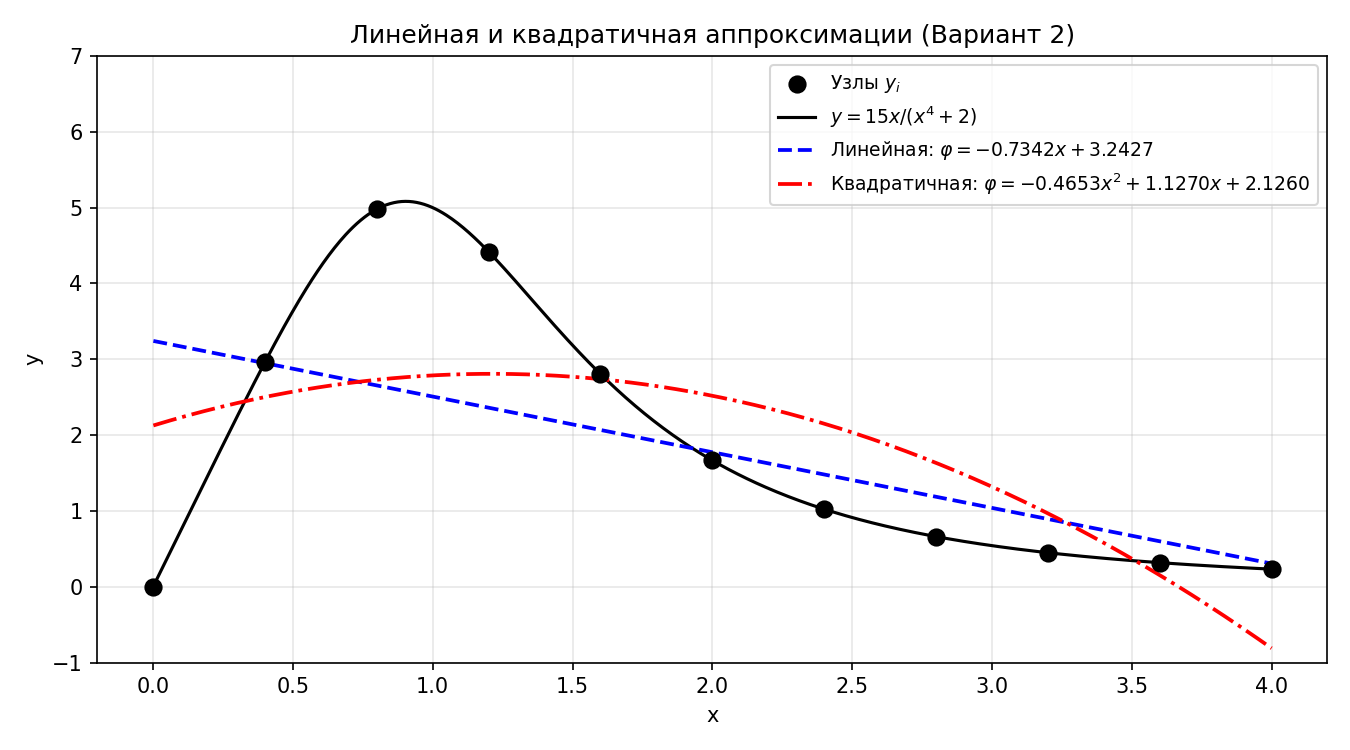
\includegraphics[width=0.88\textwidth]{plot_calc}
    \caption{Линейная и квадратичная аппроксимации}
\end{figure}

% -------------------------------------------------------
\section{Программная реализация}
% -------------------------------------------------------

\subsection{Описание программы}

Программа реализована на языке Python в виде консольного приложения с интерактивным меню. Пользователь может выбрать тип аппроксимации, загрузить данные (вариант 2 по умолчанию, ручной ввод или файл), получить коэффициенты, метрики и графики.

\textbf{Реализованные методы аппроксимации:}
\begin{itemize}
    \item Линейная: $\varphi(x) = ax + b$
    \item Квадратичная: $\varphi(x) = a_0 + a_1x + a_2x^2$
    \item Кубическая: $\varphi(x) = a_0 + a_1x + a_2x^2 + a_3x^3$
    \item Экспоненциальная: $\varphi(x) = ae^{bx}$
    \item Логарифмическая: $\varphi(x) = a\ln x + b$
    \item Степенная: $\varphi(x) = ax^b$
\end{itemize}

Для решения систем нормальных уравнений реализован метод Гаусса с выбором ведущего элемента. Все аппроксимирующие функции написаны самостоятельно (без \texttt{numpy.polyfit} и аналогов).

\subsection{Листинг программы}

\begin{lstlisting}[style=intellij, caption={Решение СЛАУ методом Гаусса}]
def gauss_solve(A, b):
    n = len(b)
    M = [[A[i][j] for j in range(n)] + [b[i]] for i in range(n)]
    for col in range(n):
        max_row = max(range(col, n), key=lambda r: abs(M[r][col]))
        M[col], M[max_row] = M[max_row], M[col]
        if abs(M[col][col]) < 1e-15:
            raise ValueError("Singular matrix")
        for row in range(col + 1, n):
            factor = M[row][col] / M[col][col]
            for j in range(col, n + 1):
                M[row][j] -= factor * M[col][j]
    x = [0.0] * n
    for i in range(n - 1, -1, -1):
        x[i] = M[i][n]
        for j in range(i + 1, n):
            x[i] -= M[i][j] * x[j]
        x[i] /= M[i][i]
    return x
\end{lstlisting}

\begin{lstlisting}[style=intellij, caption={Полиномиальная аппроксимация МНК (общий случай)}]
def lsq_polynomial(xs, ys, degree):
    n = len(xs)
    m = degree
    A = [[0.0] * (m + 1) for _ in range(m + 1)]
    b = [0.0] * (m + 1)
    for i in range(m + 1):
        for j in range(m + 1):
            A[i][j] = sum(xs[k] ** (i + j) for k in range(n))
        b[i] = sum(ys[k] * xs[k] ** i for k in range(n))
    return gauss_solve(A, b)

def poly_eval(coeffs, x):
    return sum(coeffs[i] * x ** i for i in range(len(coeffs)))
\end{lstlisting}

\begin{lstlisting}[style=intellij, caption={Линеаризация нелинейных функций}]
def lsq_exponential(xs, ys):
    # phi = a * e^(b*x) => ln(y) = ln(a) + b*x
    filtered = [(x, y) for x, y in zip(xs, ys) if y > 0]
    xs_f = [p[0] for p in filtered]
    ys_f = [math.log(p[1]) for p in filtered]
    coeffs = lsq_polynomial(xs_f, ys_f, 1)
    return math.exp(coeffs[0]), coeffs[1]

def lsq_power(xs, ys):
    # phi = a * x^b => ln(y) = ln(a) + b*ln(x)
    filtered = [(x, y) for x, y in zip(xs, ys) if x > 0 and y > 0]
    xs_f = [math.log(p[0]) for p in filtered]
    ys_f = [math.log(p[1]) for p in filtered]
    coeffs = lsq_polynomial(xs_f, ys_f, 1)
    return math.exp(coeffs[0]), coeffs[1]

def lsq_logarithmic(xs, ys):
    # phi = a*ln(x) + b => X = ln(x), Y = y
    filtered = [(x, y) for x, y in zip(xs, ys) if x > 0]
    xs_f = [math.log(p[0]) for p in filtered]
    ys_f = [p[1] for p in filtered]
    coeffs = lsq_polynomial(xs_f, ys_f, 1)
    return coeffs[1], coeffs[0]  # a, b
\end{lstlisting}

\begin{lstlisting}[style=intellij, caption={Метрики качества аппроксимации}]
def compute_metrics(xs, ys, phi_vals):
    n = len(xs)
    eps = [phi_vals[i] - ys[i] for i in range(n)]
    S = sum(e ** 2 for e in eps)
    delta = math.sqrt(S / n)
    phi_mean = sum(phi_vals) / n
    ss_res = sum((ys[i] - phi_vals[i]) ** 2 for i in range(n))
    ss_tot = sum((ys[i] - phi_mean) ** 2 for i in range(n))
    R2 = 1 - ss_res / ss_tot if ss_tot > 1e-15 else 0.0
    return S, delta, R2, eps

def pearson_r(xs, ys):
    n = len(xs)
    x_mean = sum(xs) / n
    y_mean = sum(ys) / n
    num = sum((xs[i] - x_mean) * (ys[i] - y_mean) for i in range(n))
    den = math.sqrt(sum((xs[i] - x_mean) ** 2 for i in range(n)) *
                    sum((ys[i] - y_mean) ** 2 for i in range(n)))
    return num / den if den > 1e-15 else 0.0
\end{lstlisting}

\subsection{Результаты выполнения программы}

\subsubsection{Тест 1: Данные варианта 2}

Запуск с данными варианта 2 ($n=11$ точек, $x \in [0{,}4]$, $h=0{,}4$).
Результаты сравнения всех функций:

\begin{table}[H]
\centering
\begin{tabular}{|l|r|r|r|l|}
\hline
\textbf{Функция} & \textbf{$S$} & \textbf{$\delta$} & \textbf{$R^2$} & \textbf{Качество} \\
\hline
Линейная            & 21.473987 & 1.397205 & 0.306409 & недостаточно \\
Квадратичная        & 16.718797 & 1.232838 & 0.459997 & недостаточно \\
Кубическая          &  3.967599 & 0.600575 & 0.871850 & удовлетворительно \\
Экспоненциальная    & 84.635669 & 2.773833 & $-1.26$ & недостаточно \\
Логарифмическая     &  9.561484 & 0.977828 & 0.652276 & слабая \\
Степенная           & 40.290762 & 2.007256 & $-0.47$ & недостаточно \\
\hline
\multicolumn{5}{|l|}{\textbf{Наилучшая аппроксимация: Кубическая} ($\delta = 0{,}601$)} \\
\hline
\end{tabular}
\caption{Сравнение аппроксимаций, вариант 2}
\end{table}

Кубическая аппроксимация: $\varphi(x) = 0{,}4905 + 7{,}6238\,x - 4{,}7246\,x^2 + 0{,}7099\,x^3$.

\begin{figure}[H]
    \centering
    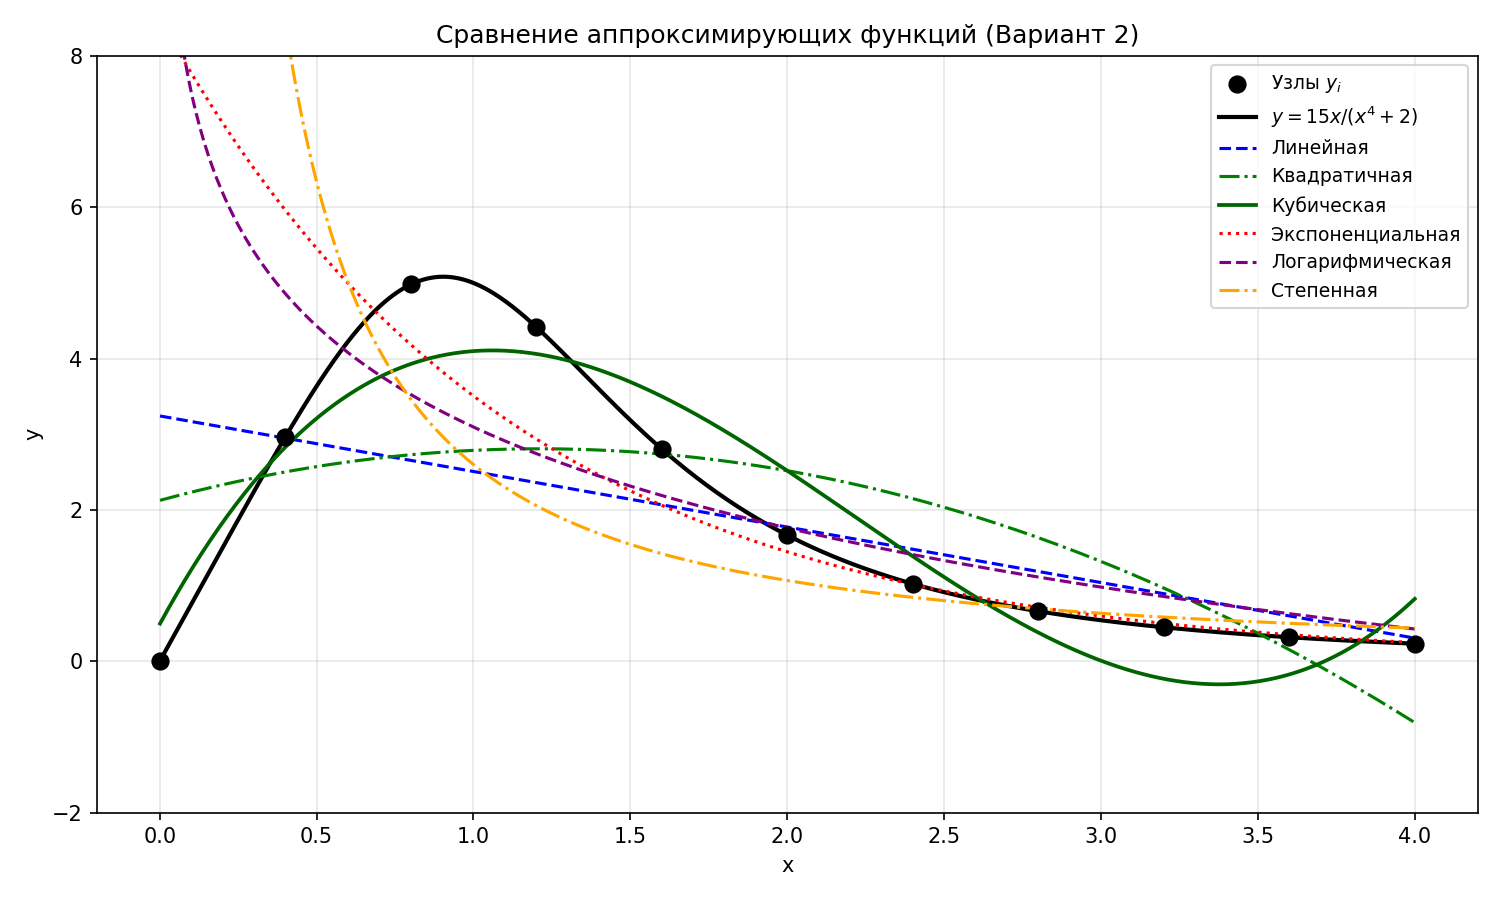
\includegraphics[width=0.88\textwidth]{plot_all}
    \caption{Все аппроксимирующие функции для варианта 2}
\end{figure}

\begin{figure}[H]
    \centering
    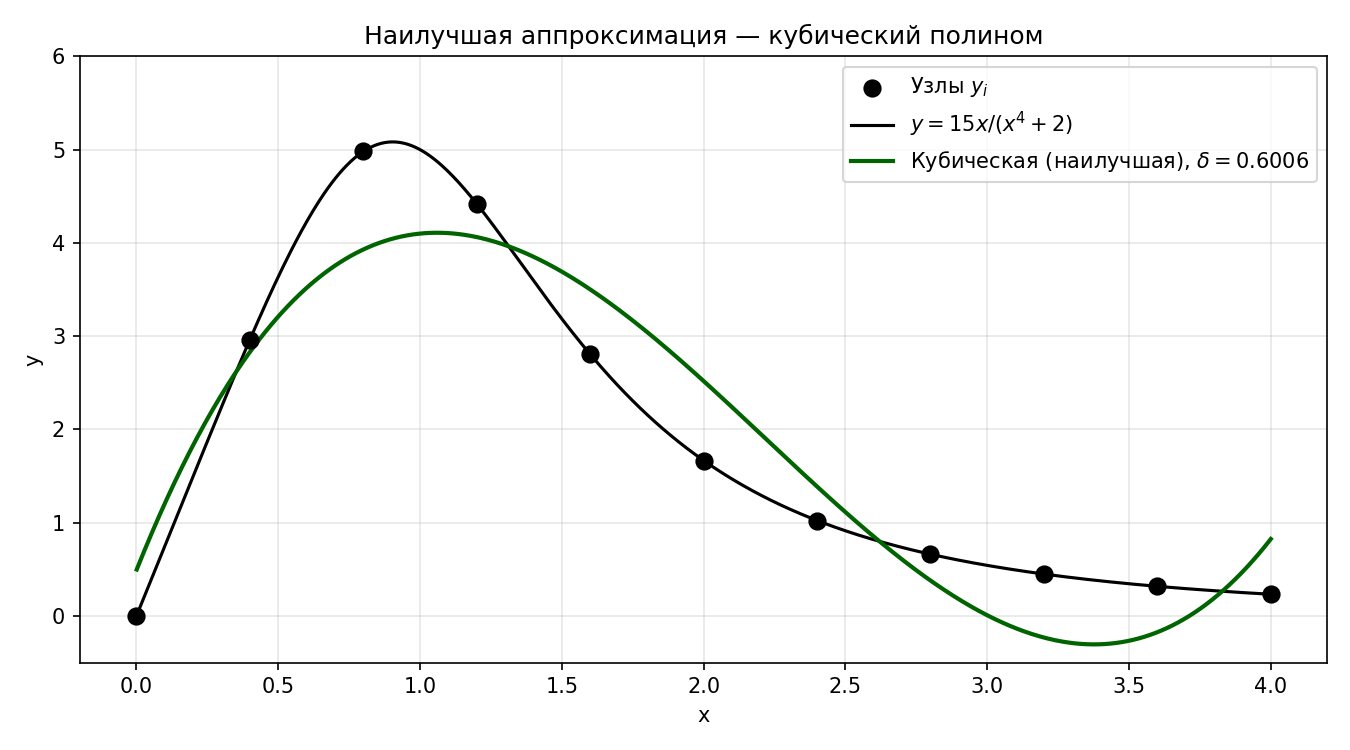
\includegraphics[width=0.82\textwidth]{plot_best}
    \caption{Наилучшая аппроксимация — кубический полином}
\end{figure}

\subsubsection{Тест 2: Линейные данные}

Данные: $\{(1, 2), (2, 4), (3, 6), (4, 8), (5, 10), (6, 12), (7, 14), (8, 16)\}$ — точная линейная зависимость.

Ожидаемый результат: линейная функция $\varphi(x) = 2x + 0$ даёт $\delta = 0$, $R^2 = 1$.
Программа выводит: $a = 2{,}0000$, $b = 0{,}0000$, $\delta \approx 0{,}000000$, $R^2 \approx 1{,}000000$.
Коэффициент корреляции Пирсона: $r = 1{,}0000$ (строгая линейная связь).

\subsubsection{Тест 3: Некорректные данные}

При попытке аппроксимировать экспоненциальной функцией данные с отрицательными значениями $y$, программа выводит сообщение:
\begin{verbatim}
Ошибка: Недостаточно точек с y > 0 для экспоненциальной аппроксимации
\end{verbatim}
и продолжает работу.

% -------------------------------------------------------
\section{Выводы}
% -------------------------------------------------------

\begin{enumerate}
    \item Для функции $y = 15x/(x^4+2)$ на отрезке $[0, 4]$ был построен ряд аппроксимирующих функций методом наименьших квадратов.

    \item Линейная и квадратичная аппроксимации показали неудовлетворительные результаты ($R^2 < 0{,}5$), так как исходная функция имеет выраженный максимум в районе $x \approx 0{,}8$ и монотонно убывает к нулю — такое поведение невозможно описать прямой или обычной параболой.

    \item Наилучшим приближением оказался \textbf{кубический полином} с $\delta = 0{,}601$ и $R^2 = 0{,}872$ (удовлетворительная аппроксимация).

    \item Экспоненциальная и степенная функции показали худшие результаты ($R^2 < 0$), что объясняется монотонным характером этих функций, не способных воспроизвести «горб» исходных данных.

    \item Разработанное консольное приложение на Python реализует метод наименьших квадратов для 6 классов функций с самостоятельно написанными алгоритмами (без \texttt{numpy.polyfit}), поддерживает ввод данных из консоли и файла, вычисляет все требуемые метрики и строит графики.
\end{enumerate}

\end{document}